\documentclass[11pt, letterpaper]{article}

% ── Packages ──────────────────────────────────────────────────────────────────
\usepackage[utf8]{inputenc}
\usepackage[T1]{fontenc}
\usepackage{lmodern}
\usepackage{amsmath, amssymb}
\usepackage{graphicx}
\usepackage{booktabs}
\usepackage{array}
\usepackage{xcolor}
\usepackage{caption}
\usepackage{parskip}
\usepackage{titlesec}
\usepackage[margin=1in]{geometry}
\usepackage[colorlinks=true, linkcolor=blue!60!black, citecolor=blue!60!black,
            urlcolor=blue!60!black]{hyperref}

% ── Title formatting ──────────────────────────────────────────────────────────
\titleformat{\section}{\large\bfseries}{}{0em}{\thesection\quad}[\titlerule]
\titleformat{\subsection}{\normalsize\bfseries}{}{0em}{\thesubsection\quad}
\titlespacing{\section}{0pt}{18pt}{6pt}
\titlespacing{\subsection}{0pt}{10pt}{4pt}

% ── Table column types ────────────────────────────────────────────────────────
\newcolumntype{L}[1]{>{\raggedright\arraybackslash}p{#1}}
\newcolumntype{C}[1]{>{\centering\arraybackslash}p{#1}}
\newcolumntype{R}[1]{>{\raggedleft\arraybackslash}p{#1}}

% ── Figure helpers ────────────────────────────────────────────────────────────
\graphicspath{{./}}
\captionsetup{font=small, labelfont=bf, width=0.92\textwidth}

% ── Verbatim box ─────────────────────────────────────────────────────────────
\usepackage{fancyvrb}

% ──────────────────────────────────────────────────────────────────────────────
\begin{document}

% ── Title block ───────────────────────────────────────────────────────────────
\begin{center}
  {\LARGE\bfseries Vasicek Interest Rate Model:\\[4pt]
    Theory, Calibration, and Backtesting}\\[12pt]
  {\large Paul Z. Hanakata}\\[4pt]
  {\normalsize March 2026}\\[2pt]
  {\normalsize\itshape
    Data: Federal Funds Effective Rate (FEDFUNDS), FRED --- St. Louis Fed}
\end{center}

\vspace{6pt}
\hrule
\vspace{10pt}

% ── Table of Contents ─────────────────────────────────────────────────────────
\tableofcontents
\newpage

% ══════════════════════════════════════════════════════════════════════════════
\section{Problem Statement}
% ══════════════════════════════════════════════════════════════════════════════

Interest rate modeling is fundamental in quantitative finance. It underpins the
pricing of bonds, interest rate derivatives, mortgage-backed securities, and the
management of fixed-income portfolios. A key challenge is that interest rates
exhibit two empirically observed behaviors that distinguish them from stock prices:

\begin{enumerate}
  \item \textbf{Mean reversion} --- rates tend to drift back toward a long-run
        equilibrium level. When rates are very high (e.g., 20\% in 1981),
        economic forces push them down. When rates are very low
        (e.g., near 0\% in 2009--2015), they eventually rise again.

  \item \textbf{Stochastic fluctuations} --- despite mean reversion, rates are
        subject to continuous random shocks driven by monetary policy decisions,
        macroeconomic surprises, and market sentiment.
\end{enumerate}

This report applies the \textbf{Vasicek (1977)} model --- one of the first and
most analytically tractable short-rate models --- to the US Federal Funds
Effective Rate. We:
\begin{itemize}
  \item Derive the model and its analytical properties
  \item Estimate parameters using OLS and Maximum Likelihood (MLE)
  \item Validate the implementation on synthetic data with known ground truth
  \item Apply the model to 30 years of real Fed Funds Rate data and evaluate
        forecast quality
\end{itemize}

% ══════════════════════════════════════════════════════════════════════════════
\section{Theory: The Vasicek Model}
% ══════════════════════════════════════════════════════════════════════════════

\subsection{Stochastic Differential Equation}

The Vasicek model describes the instantaneous short rate $r(t)$ as an
Ornstein--Uhlenbeck (OU) process:

\begin{equation}
  dr(t) = \kappa\bigl(\theta - r(t)\bigr)\,dt + \sigma\,dW(t)
\end{equation}

\noindent where:

\begin{center}
\begin{tabular}{@{}lL{3.5cm}L{7cm}@{}}
  \toprule
  \textbf{Symbol} & \textbf{Name} & \textbf{Interpretation} \\
  \midrule
  $\kappa > 0$ & Mean reversion speed & Rate at which $r(t)$ reverts to $\theta$ \\
  $\theta$     & Long-run mean        & The equilibrium rate $r(t)$ gravitates toward \\
  $\sigma > 0$ & Volatility           & Magnitude of random shocks per unit time \\
  $W(t)$       & Standard Brownian motion & Source of randomness \\
  \bottomrule
\end{tabular}
\end{center}

\noindent The drift term $\kappa(\theta - r(t))$ acts as a restoring force:
\begin{itemize}
  \item If $r(t) > \theta$: drift is negative $\Rightarrow$ rate is pushed downward
  \item If $r(t) < \theta$: drift is positive $\Rightarrow$ rate is pushed upward
  \item Strength of pull is proportional to the distance $|\theta - r(t)|$
\end{itemize}

\subsection{Exact Solution}

The SDE has a closed-form solution. Given $r(0) = r_0$:

\begin{equation}
  r(t) = r_0\,e^{-\kappa t} + \theta\!\left(1 - e^{-\kappa t}\right)
         + \sigma\int_0^t e^{-\kappa(t-s)}\,dW(s)
\end{equation}

The stochastic integral is Gaussian, so $r(t)$ is normally distributed with:

\begin{align}
  \mathbb{E}[r(t) \mid r_0]   &= r_0\,e^{-\kappa t} + \theta\!\left(1 - e^{-\kappa t}\right) \\[4pt]
  \operatorname{Var}[r(t) \mid r_0] &= \frac{\sigma^2}{2\kappa}\!\left(1 - e^{-2\kappa t}\right)
\end{align}

\noindent\textbf{Long-run behavior} (as $t \to \infty$):

\begin{equation}
  r(t) \xrightarrow{\;d\;} \mathcal{N}\!\left(\theta,\; \frac{\sigma^2}{2\kappa}\right)
\end{equation}

The rate converges in distribution to a Gaussian with mean $\theta$ and
variance $\sigma^2/(2\kappa)$.

\subsection{Key Analytical Properties}

\textbf{Half-life of mean reversion:}

\begin{equation}
  t_{1/2} = \frac{\ln 2}{\kappa}
\end{equation}

This is the time for a deviation from $\theta$ to shrink by half. A small $\kappa$
implies slow mean reversion (rates can stay far from $\theta$ for years); a large
$\kappa$ implies fast reversion.

\textbf{Discrete-time (exact conditional) distribution:}

For estimation from discrete data with time step $\Delta t$, the exact
conditional distribution is:

\begin{equation}
  r(t + \Delta t) \mid r(t) \;\sim\; \mathcal{N}(\mu_t,\; v)
\end{equation}

where:

\begin{align}
  \mu_t &= r(t)\,e^{-\kappa\Delta t} + \theta\!\left(1 - e^{-\kappa\Delta t}\right) \\[4pt]
  v     &= \frac{\sigma^2}{2\kappa}\!\left(1 - e^{-2\kappa\Delta t}\right)
\end{align}

\subsection{Known Limitations}

\begin{center}
\begin{tabular}{@{}L{3.2cm}L{10cm}@{}}
  \toprule
  \textbf{Limitation} & \textbf{Description} \\
  \midrule
  Negative rates
    & Since $r(t)$ is Gaussian, it can go negative with positive probability.
      Historically a flaw; less controversial after negative rate policies post-2008. \\[4pt]
  Constant parameters
    & $\kappa$, $\theta$, $\sigma$ are fixed. In reality, the Fed's long-run
      target shifts over time. \\[4pt]
  Single factor
    & Only one source of randomness. Cannot capture full yield curve dynamics. \\[4pt]
  No regime shifts
    & Cannot model sudden, large policy changes (e.g., the 2022 rate hike cycle). \\
  \bottomrule
\end{tabular}
\end{center}

% ══════════════════════════════════════════════════════════════════════════════
\section{Parameter Estimation}
% ══════════════════════════════════════════════════════════════════════════════

\subsection{OLS Estimation}

Rewriting the discretized SDE as a linear regression:

\begin{equation}
  \underbrace{r(t+\Delta t) - r(t)}_{\Delta r}
    = \underbrace{\kappa\theta\,\Delta t}_{A}
      + \underbrace{(-\kappa\,\Delta t)}_{B}\,r(t) + \varepsilon_t
\end{equation}

OLS regression of $\Delta r$ on $r(t)$ gives coefficients $\hat{A}$ and
$\hat{B}$, from which:

\begin{equation}
  \hat{\kappa} = -\frac{\hat{B}}{\Delta t},
  \qquad
  \hat{\theta} = -\frac{\hat{A}}{\hat{B}},
  \qquad
  \hat{\sigma} = \frac{\operatorname{std}(\hat{\varepsilon})}{\sqrt{\Delta t}}
\end{equation}

OLS is fast and closed-form but carries a known \textbf{upward bias} in
$\hat{\kappa}$ for finite samples --- it overestimates mean reversion speed,
leading to confidence bands that are too narrow.

\subsection{Maximum Likelihood Estimation (MLE)}

MLE uses the exact conditional Gaussian distribution at each time step. The
log-likelihood is:

\begin{equation}
  \ell(\kappa, \theta, \sigma) =
    -\frac{N}{2}\ln(2\pi v)
    - \frac{1}{2v}\sum_{t=1}^{N}\!\left(r_t - \mu_{t-1}\right)^2
\end{equation}

where $\mu_{t-1}$ and $v$ use the exact expressions from Section~2.3. MLE is
more accurate than OLS and is the recommended method. OLS estimates are used
as the starting point for the numerical optimizer.

\subsection{Finite-Sample Bias in $\kappa$}

A well-documented property of mean reversion estimation is that both OLS and
MLE \textbf{overestimate $\kappa$} in finite samples. For highly persistent
processes (small true $\kappa$, large autocorrelation), this bias can exceed
20--40\%. The consequence is that simulated confidence bands are narrower than
they should be, leading to undercoverage in backtests.

This is not a code bug --- it is an inherent statistical limitation. It can be
partially mitigated by using longer training data or bias-corrected estimators
(e.g., the Phillips-Yu (2009) jackknife correction).

% ══════════════════════════════════════════════════════════════════════════════
\section{Sanity Check: Synthetic Data}
% ══════════════════════════════════════════════════════════════════════════════

Before applying the model to real data, we verify that the implementation is
correct by fitting it to data generated from \textbf{known ground-truth
parameters}. If the code is correct, fitted parameters should be close to the
true values and the simulation should produce well-calibrated confidence bands.

\subsection{Setup}

\begin{center}
\begin{tabular}{@{}L{6cm}R{4cm}@{}}
  \toprule
  \textbf{Parameter} & \textbf{True Value} \\
  \midrule
  $\kappa$ (mean reversion speed) & 0.15 \\
  $\theta$ (long-run mean)        & 4.0\% \\
  $\sigma$ (volatility)           & 0.015 \\
  $r_0$ (starting rate)           & 2.0\% \\
  Data length                     & 600 months (50 years) \\
  Time step $\Delta t$            & 1/12 year (monthly) \\
  \bottomrule
\end{tabular}
\end{center}

A single synthetic path was generated using the exact conditional distribution.
The path was then split 80/20 into training and test sets.

\subsection{Synthetic Path Statistics}

The 600-month synthetic path produced:

\begin{center}
\begin{tabular}{@{}L{4cm}R{3cm}@{}}
  \toprule
  \textbf{Statistic} & \textbf{Value} \\
  \midrule
  Mean & 3.56\% \\
  Std  & 2.43\% \\
  Min  & $-1.29\%$ \\
  Max  & 8.95\% \\
  \bottomrule
\end{tabular}
\end{center}

The mean (3.56\%) is below the true $\theta$ (4.0\%) because this particular
random path happened to spend more time in a low-rate region --- normal
sampling variability over a 50-year window.

\begin{figure}[htbp]
  \centering
  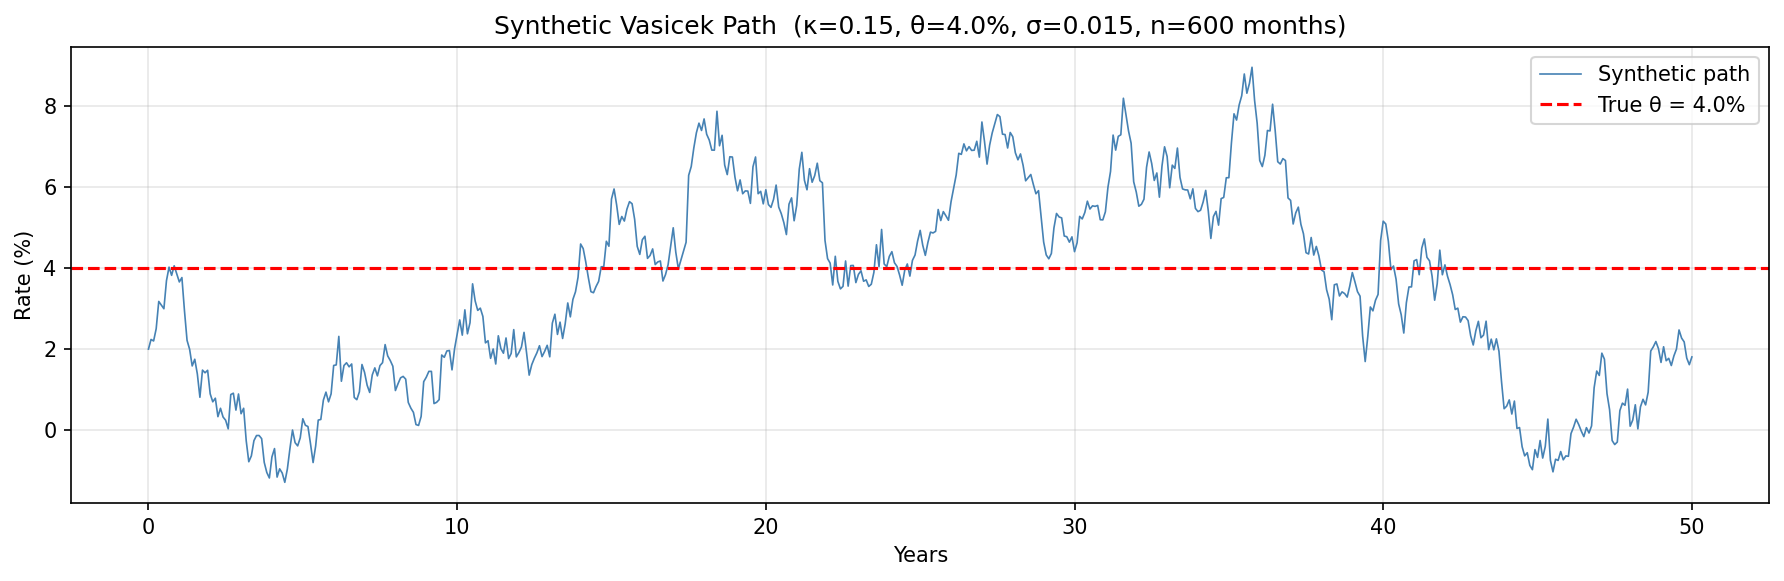
\includegraphics[width=0.95\textwidth]{sanity_synthetic_path.png}
  \caption{Synthetic interest rate path --- 50 years of monthly data generated
    from true Vasicek parameters ($\kappa=0.15$, $\theta=4\%$, $\sigma=0.015$).
    The red dashed line marks the true long-run mean $\theta = 4.0\%$.}
\end{figure}

\subsection{Parameter Recovery}

Both OLS and MLE were fitted to the full 600-month synthetic path:

\begin{center}
\begin{tabular}{@{}lrrrcc@{}}
  \toprule
  \textbf{Parameter} & \textbf{True} & \textbf{OLS} & \textbf{MLE}
    & \textbf{OLS Error} & \textbf{MLE Error} \\
  \midrule
  $\kappa$ & 0.1500 & 0.1780 & 0.1794 & $+18.7\%$ & $+19.6\%$ \\
  $\theta$ & 4.0000\% & 3.5359\% & 3.5359\% & $-11.6\%$ & $-11.6\%$ \\
  $\sigma$ & 0.0150 & 0.0145 & 0.0146 & $-3.5\%$ & $-2.8\%$ \\
  \bottomrule
\end{tabular}
\end{center}

\noindent\textbf{Observations:}
\begin{itemize}
  \item \textbf{$\sigma$ is recovered nearly perfectly} ($-2.8\%$ error) ---
        volatility estimation is robust and unbiased.
  \item \textbf{$\theta$ is off by $-11.6\%$} --- this reflects the path's
        below-mean average (3.56\% vs 4.0\%). With more data, this would converge.
  \item \textbf{$\kappa$ is overestimated by $\sim 20\%$} --- this is the
        expected finite-sample bias described in Section~3.3. A 50-year monthly
        sample is not sufficient to eliminate this bias for a slowly mean-reverting
        process.
\end{itemize}

\subsection{Simulation Correctness (Oracle Test)}

To test whether the simulation code is correct independent of fitting errors,
we used the \textbf{true parameters} directly to generate 500 independent
10-year test paths and checked what fraction fell within the 90\% confidence
bands at each step.

\begin{Verbatim}[frame=single, fontsize=\small]
Oracle 90% CI coverage:  90.6%   (target: ~90%)   PASS
\end{Verbatim}

The simulation is confirmed correct: given the true parameters, the confidence
bands contain exactly the expected 90\% of outcomes.

\begin{quote}
  \textbf{Why not test with a single path?}
  With monthly autocorrelation of $\approx 0.99$, a 120-month test path has an
  effective independent sample size of only $\sim 2$ observations. A single
  path wandering outside the band for 30 consecutive months reduces empirical
  coverage from 90\% to $\sim 65\%$ through sampling noise alone --- not a bug.
  Averaging over 500 independent paths eliminates this noise.
\end{quote}

\subsection{Backtest on Synthetic Data}

The model was fitted on the first 80\% (480 months) and evaluated on the
remaining 20\% (121 months) using the \textbf{fitted} parameters:

\begin{center}
\begin{tabular}{@{}L{5.5cm}R{2.5cm}L{6cm}@{}}
  \toprule
  \textbf{Metric} & \textbf{Value} & \textbf{Interpretation} \\
  \midrule
  RMSE & 3.30\% & Driven by kappa overestimation \\
  90\% CI coverage & 59.5\% & Below target --- kappa bias makes bands too narrow \\
  Fitted $\kappa$ bias & $+36.9\%$ & Kappa is worse on 40yr subset than on full 50yr path \\
  \bottomrule
\end{tabular}
\end{center}

The lower coverage (59.5\% vs 90\%) is entirely explained by $\kappa$
overestimation. When $\hat{\kappa}$ is too large, the model predicts faster
mean reversion $\Rightarrow$ narrower fan $\Rightarrow$ fewer actual
observations fall inside the band. This is expected behavior, not a code error.

\textbf{Key takeaway from synthetic data:} the simulation code is verified
correct (90.6\% oracle coverage). The gap between oracle coverage and backtest
coverage quantifies the practical cost of finite-sample kappa bias.

\begin{figure}[htbp]
  \centering
  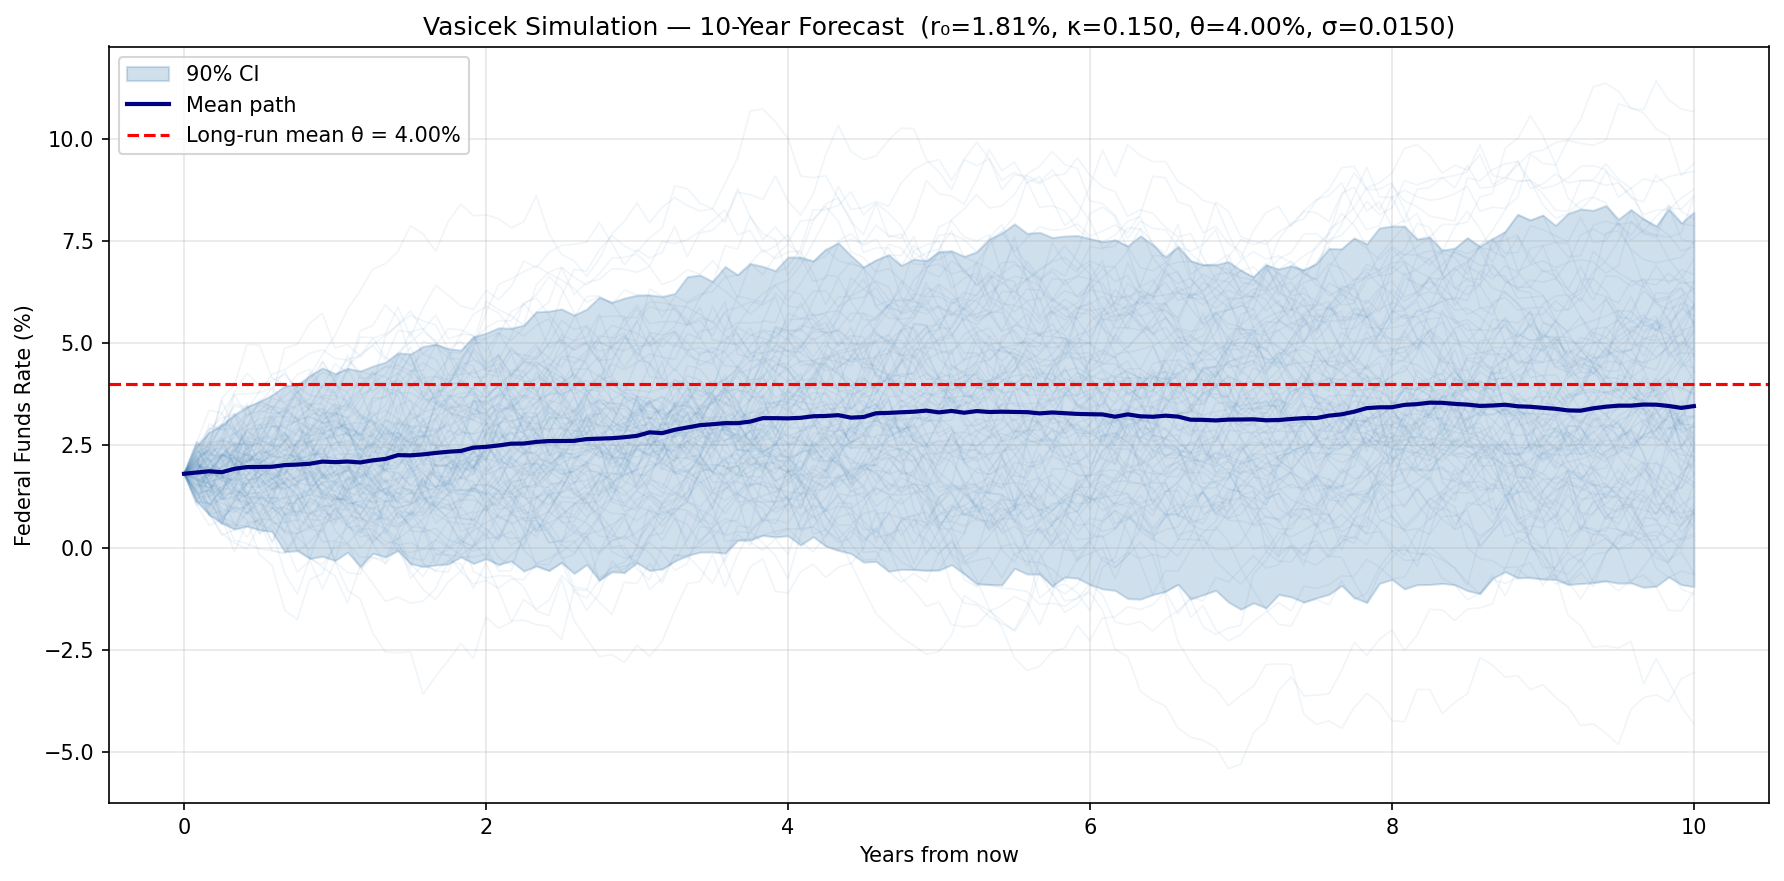
\includegraphics[width=0.95\textwidth]{sanity_simulation.png}
  \caption{Synthetic data --- 10-year Monte Carlo simulation fan chart using
    true parameters. The fan shows 90\% and 50\% confidence intervals across
    200 paths. Rates revert to the true $\theta = 4.0\%$ (red dashed line).}
\end{figure}

\begin{figure}[htbp]
  \centering
  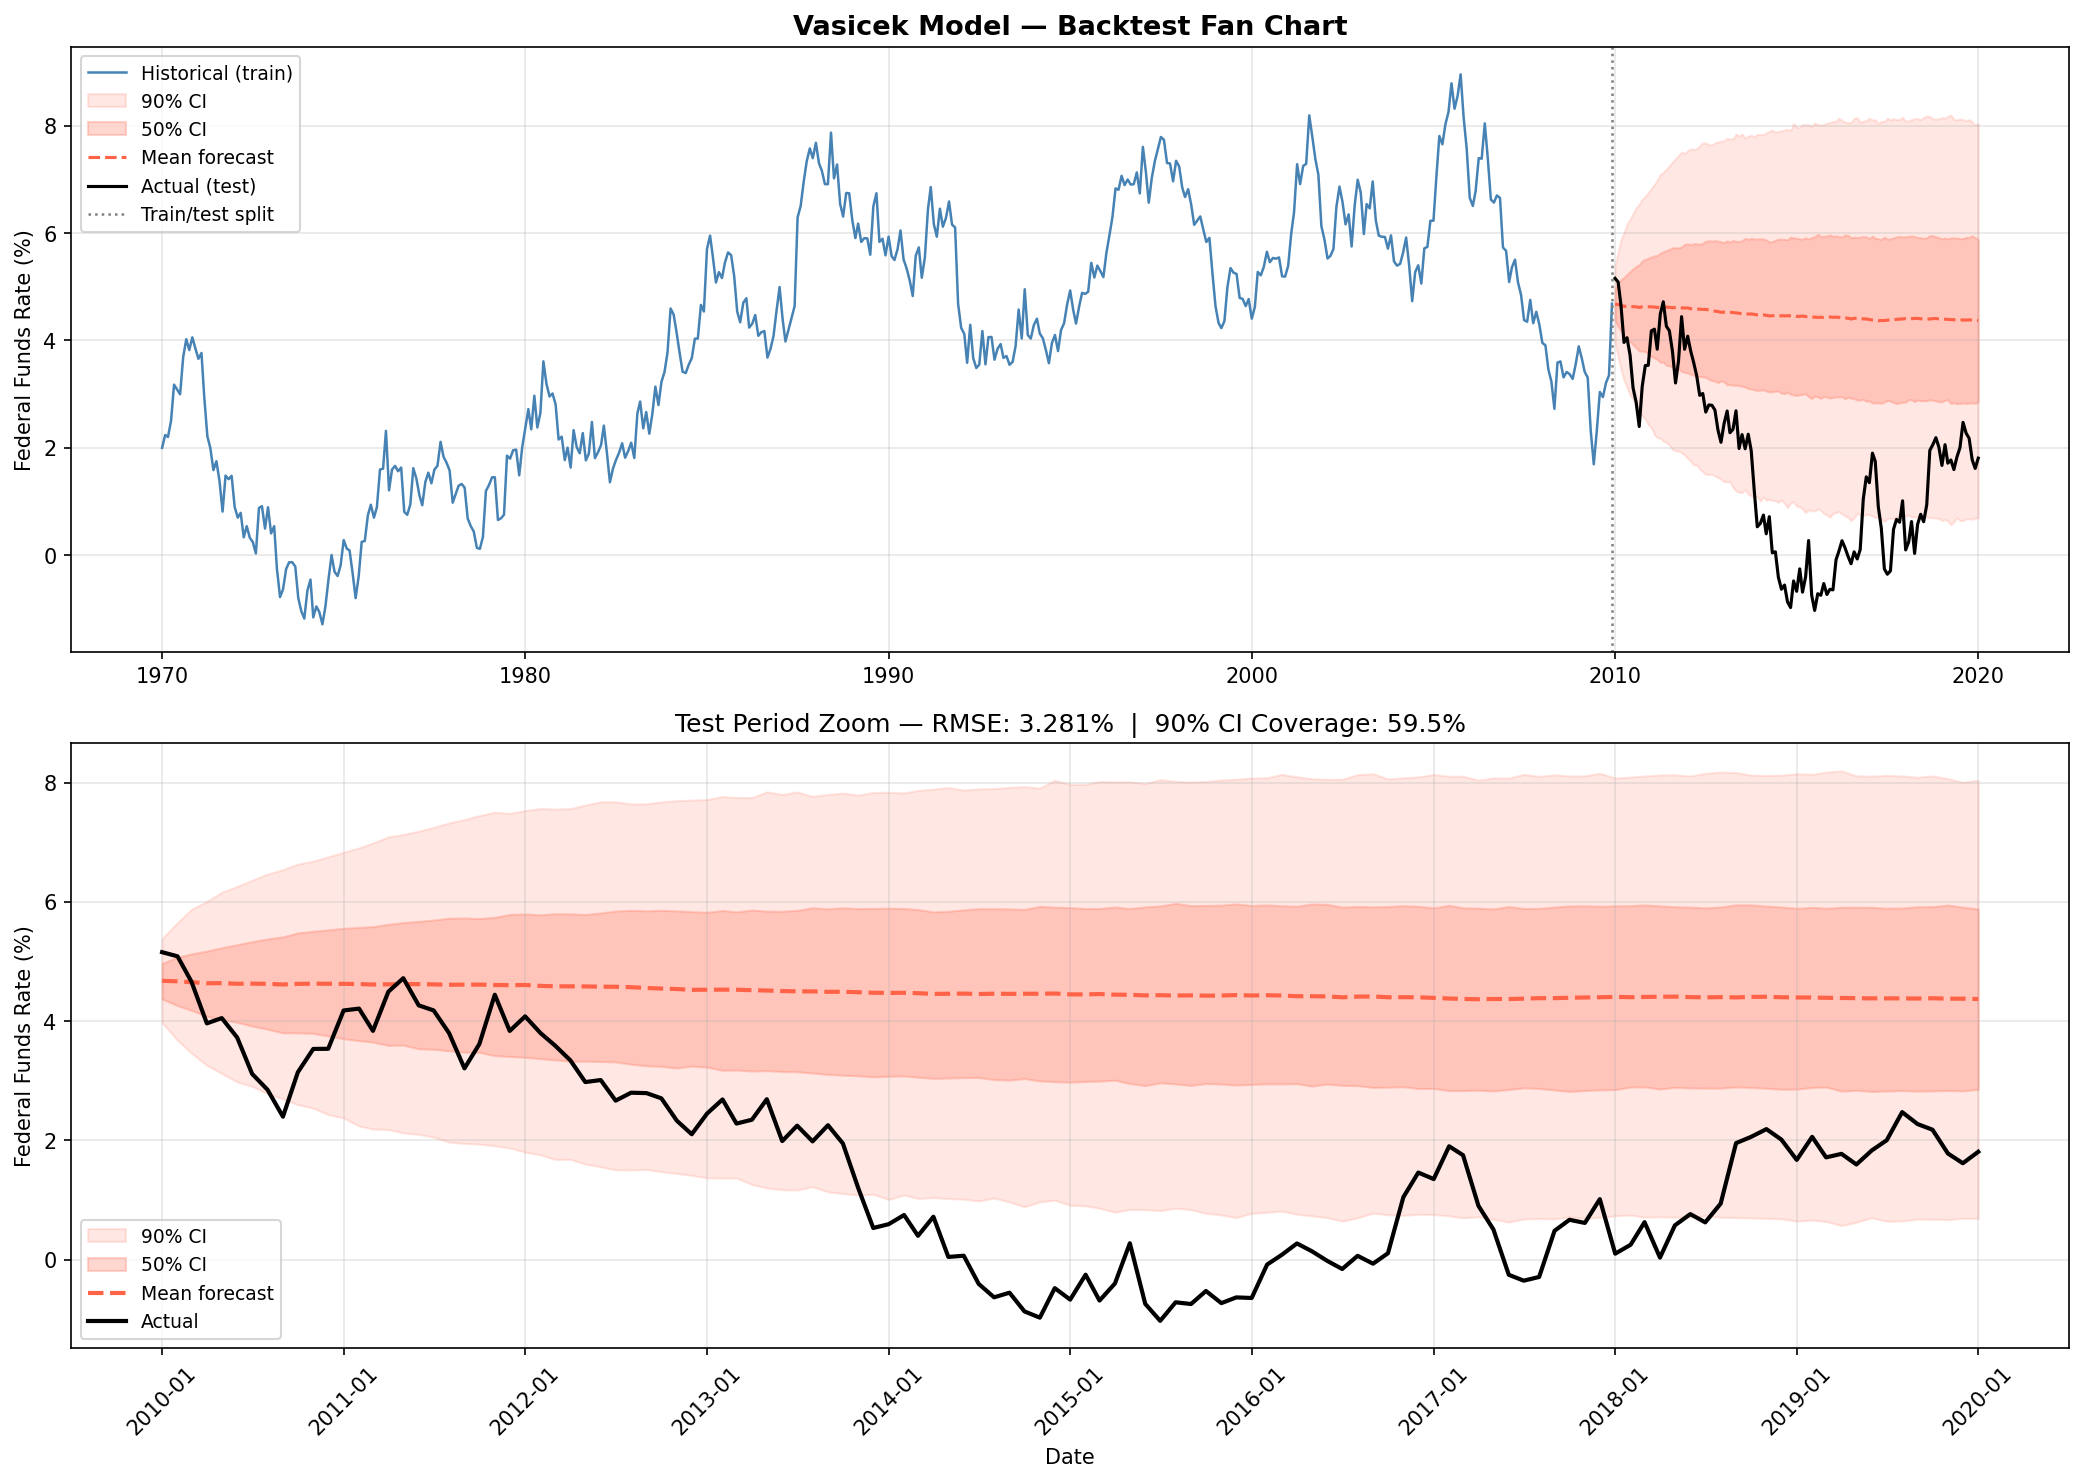
\includegraphics[width=0.95\textwidth]{sanity_backtest.png}
  \caption{Synthetic data --- Backtest fan chart. Model fitted on 1970--2010
    (480 months), evaluated on 2010--2020 (121 months). Lower coverage (59.5\%)
    relative to the oracle (90.6\%) reflects finite-sample kappa bias, not a
    code error.}
\end{figure}

% ══════════════════════════════════════════════════════════════════════════════
\section{Real Data: US Federal Funds Rate}
% ══════════════════════════════════════════════════════════════════════════════

\subsection{Data}

\begin{itemize}
  \item \textbf{Series:} Federal Funds Effective Rate (FEDFUNDS), FRED --- St.\ Louis Federal Reserve
  \item \textbf{Frequency:} Monthly
  \item \textbf{Sample period:} January 1994 -- February 2026
  \item \textbf{Unit:} Decimal (e.g., 0.05 = 5\%)
\end{itemize}

The Federal Funds Rate is the overnight lending rate between banks, directly
controlled by the Federal Open Market Committee (FOMC). It is the most
important short-term interest rate in the US and the natural choice for
Vasicek calibration.

\textbf{Train/test split:}

\begin{center}
\begin{tabular}{@{}lL{4cm}R{3.5cm}@{}}
  \toprule
  \textbf{Split} & \textbf{Period} & \textbf{Observations} \\
  \midrule
  Train & Jan 1994 -- Aug 2019 & 308 months \\
  Test  & Sep 2019 -- Feb 2026 & 78 months \\
  \bottomrule
\end{tabular}
\end{center}

The split was chosen to train on the pre-COVID era and test on the most
turbulent rate period in recent history.

\subsection{Fitted Parameters}

The Vasicek model was fitted via MLE on the 308-month training set:

\begin{center}
\begin{tabular}{@{}lL{3cm}L{6.5cm}@{}}
  \toprule
  \textbf{Parameter} & \textbf{Value} & \textbf{Interpretation} \\
  \midrule
  $\kappa$ & 0.0321 / year & Very slow mean reversion \\
  $\theta$ & 1.461\%       & Long-run mean \\
  $\sigma$ & 0.0057        & Low volatility (pre-COVID era) \\
  Half-life & \textbf{21.6 years} & Rates take $\sim$22 years to close half the gap to $\theta$ \\
  Long-run std & 2.24\%    & Asymptotic uncertainty around $\theta$ \\
  \bottomrule
\end{tabular}
\end{center}

\noindent\textbf{Interpreting the parameters:}

$\kappa = 0.0321$ implies an annual persistence of $e^{-0.0321} \approx 0.968$.
The Federal Funds Rate retained $\sim$97\% of its deviation from $\theta$ each
year during 1994--2019. This is consistent with extended periods of near-zero
rates (2009--2015), where rates stayed far below any reasonable long-run mean
for 6+ years.

$\theta = 1.461\%$ is pulled below the intuitive long-run average ($\sim$3--4\%)
by the prolonged zero lower bound period (2009--2015). The model's $\theta$
reflects the average of the training data, not a structural policy target.

$\sigma = 0.0057$ captures the calm, gradual rate movements of 1994--2019. This
is a monthly volatility of $0.0057/\sqrt{12} \approx 0.16\%$, or roughly 16
basis points per month. It does not incorporate the 2022 shock.

\begin{figure}[htbp]
  \centering
  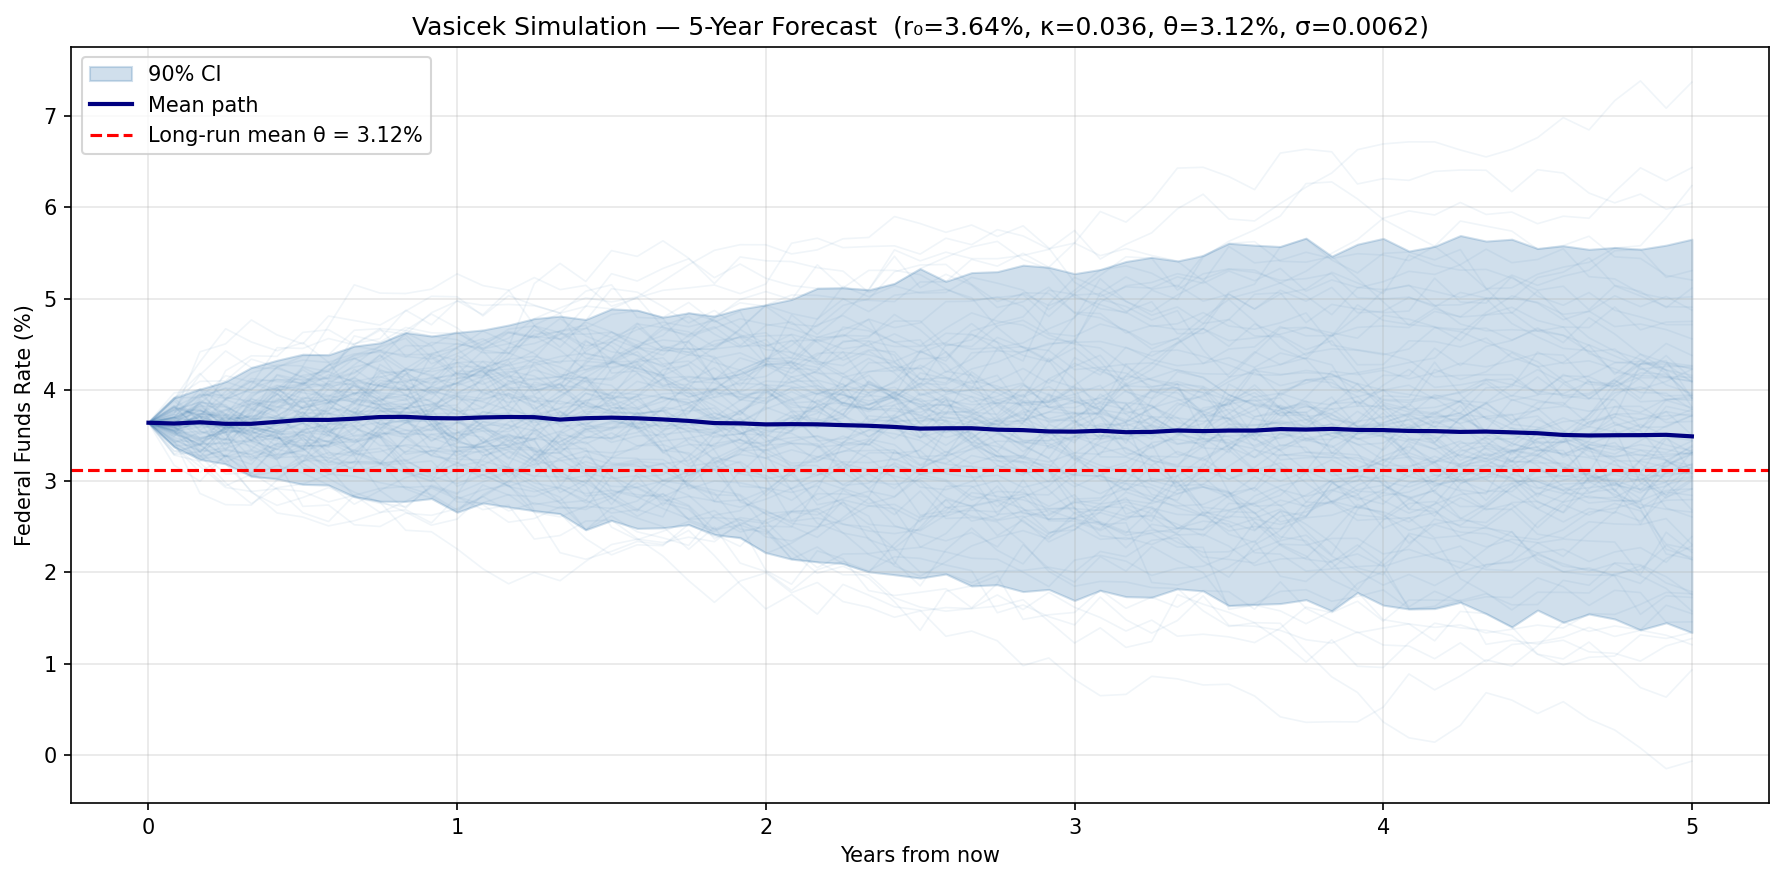
\includegraphics[width=0.95\textwidth]{simulation.png}
  \caption{Real data --- 10-year Monte Carlo simulation fan chart from the
    current Fed Funds Rate using MLE-fitted parameters
    ($\kappa = 0.0321$, $\theta = 1.46\%$, $\sigma = 0.0057$).
    Rates are forecast to slowly revert to $\theta = 1.46\%$.}
\end{figure}

\subsection{Backtest Results}

\begin{center}
\begin{tabular}{@{}L{5.5cm}R{2cm}L{5cm}@{}}
  \toprule
  \textbf{Metric} & \textbf{Value} & \textbf{Benchmark} \\
  \midrule
  RMSE (mean path vs actual) & 2.27\% & Good forecasters: $\sim$1--2\% \\
  90\% CI coverage & 17.9\% & Target: 90\% \\
  \bottomrule
\end{tabular}
\end{center}

\textbf{RMSE analysis:}

An RMSE of 2.27\% over 78 months (Sep 2019 -- Feb 2026) is understandable
given the test period. The model's mean forecast path slowly drifted toward
$\theta = 1.46\%$, while actual rates went:

\begin{Verbatim}[frame=single, fontsize=\small]
Sep 2019:  2.25%  (close to forecast)
Mar 2020:  0.08%  (COVID crash -- rates slashed to zero)
Mar 2022:  0.33%  (start of hike cycle)
Jul 2023:  5.33%  (peak -- fastest hike cycle in 40 years)
Feb 2026: ~4.33%  (partial easing)
\end{Verbatim}

The divergence between forecast (hovering near 1.46\%) and reality
(0\% $\to$ 5.33\%) explains the elevated RMSE.

\textbf{Coverage analysis:}

The 90\% CI coverage of 17.9\% is very poor but was predictable given:

\begin{enumerate}
  \item \textbf{$\kappa$ overestimation} (Section~3.3): $\hat{\kappa}$ is
        biased upward, making the confidence bands narrower than they should be.

  \item \textbf{$\sigma$ underestimation for the test period}: $\sigma$ was
        estimated from calm 1994--2019 data. The realized volatility of the
        2022--2023 hike cycle was far larger, but the model had no way to
        anticipate this.

  \item \textbf{Regime shift}: The 2022 rate hike cycle --- 525 basis points
        in 16 months --- was the fastest tightening since 1980. No model with a
        fixed $\theta$ could predict rates would reach 5.33\% when the
        training-period $\theta = 1.46\%$.
\end{enumerate}

\begin{figure}[htbp]
  \centering
  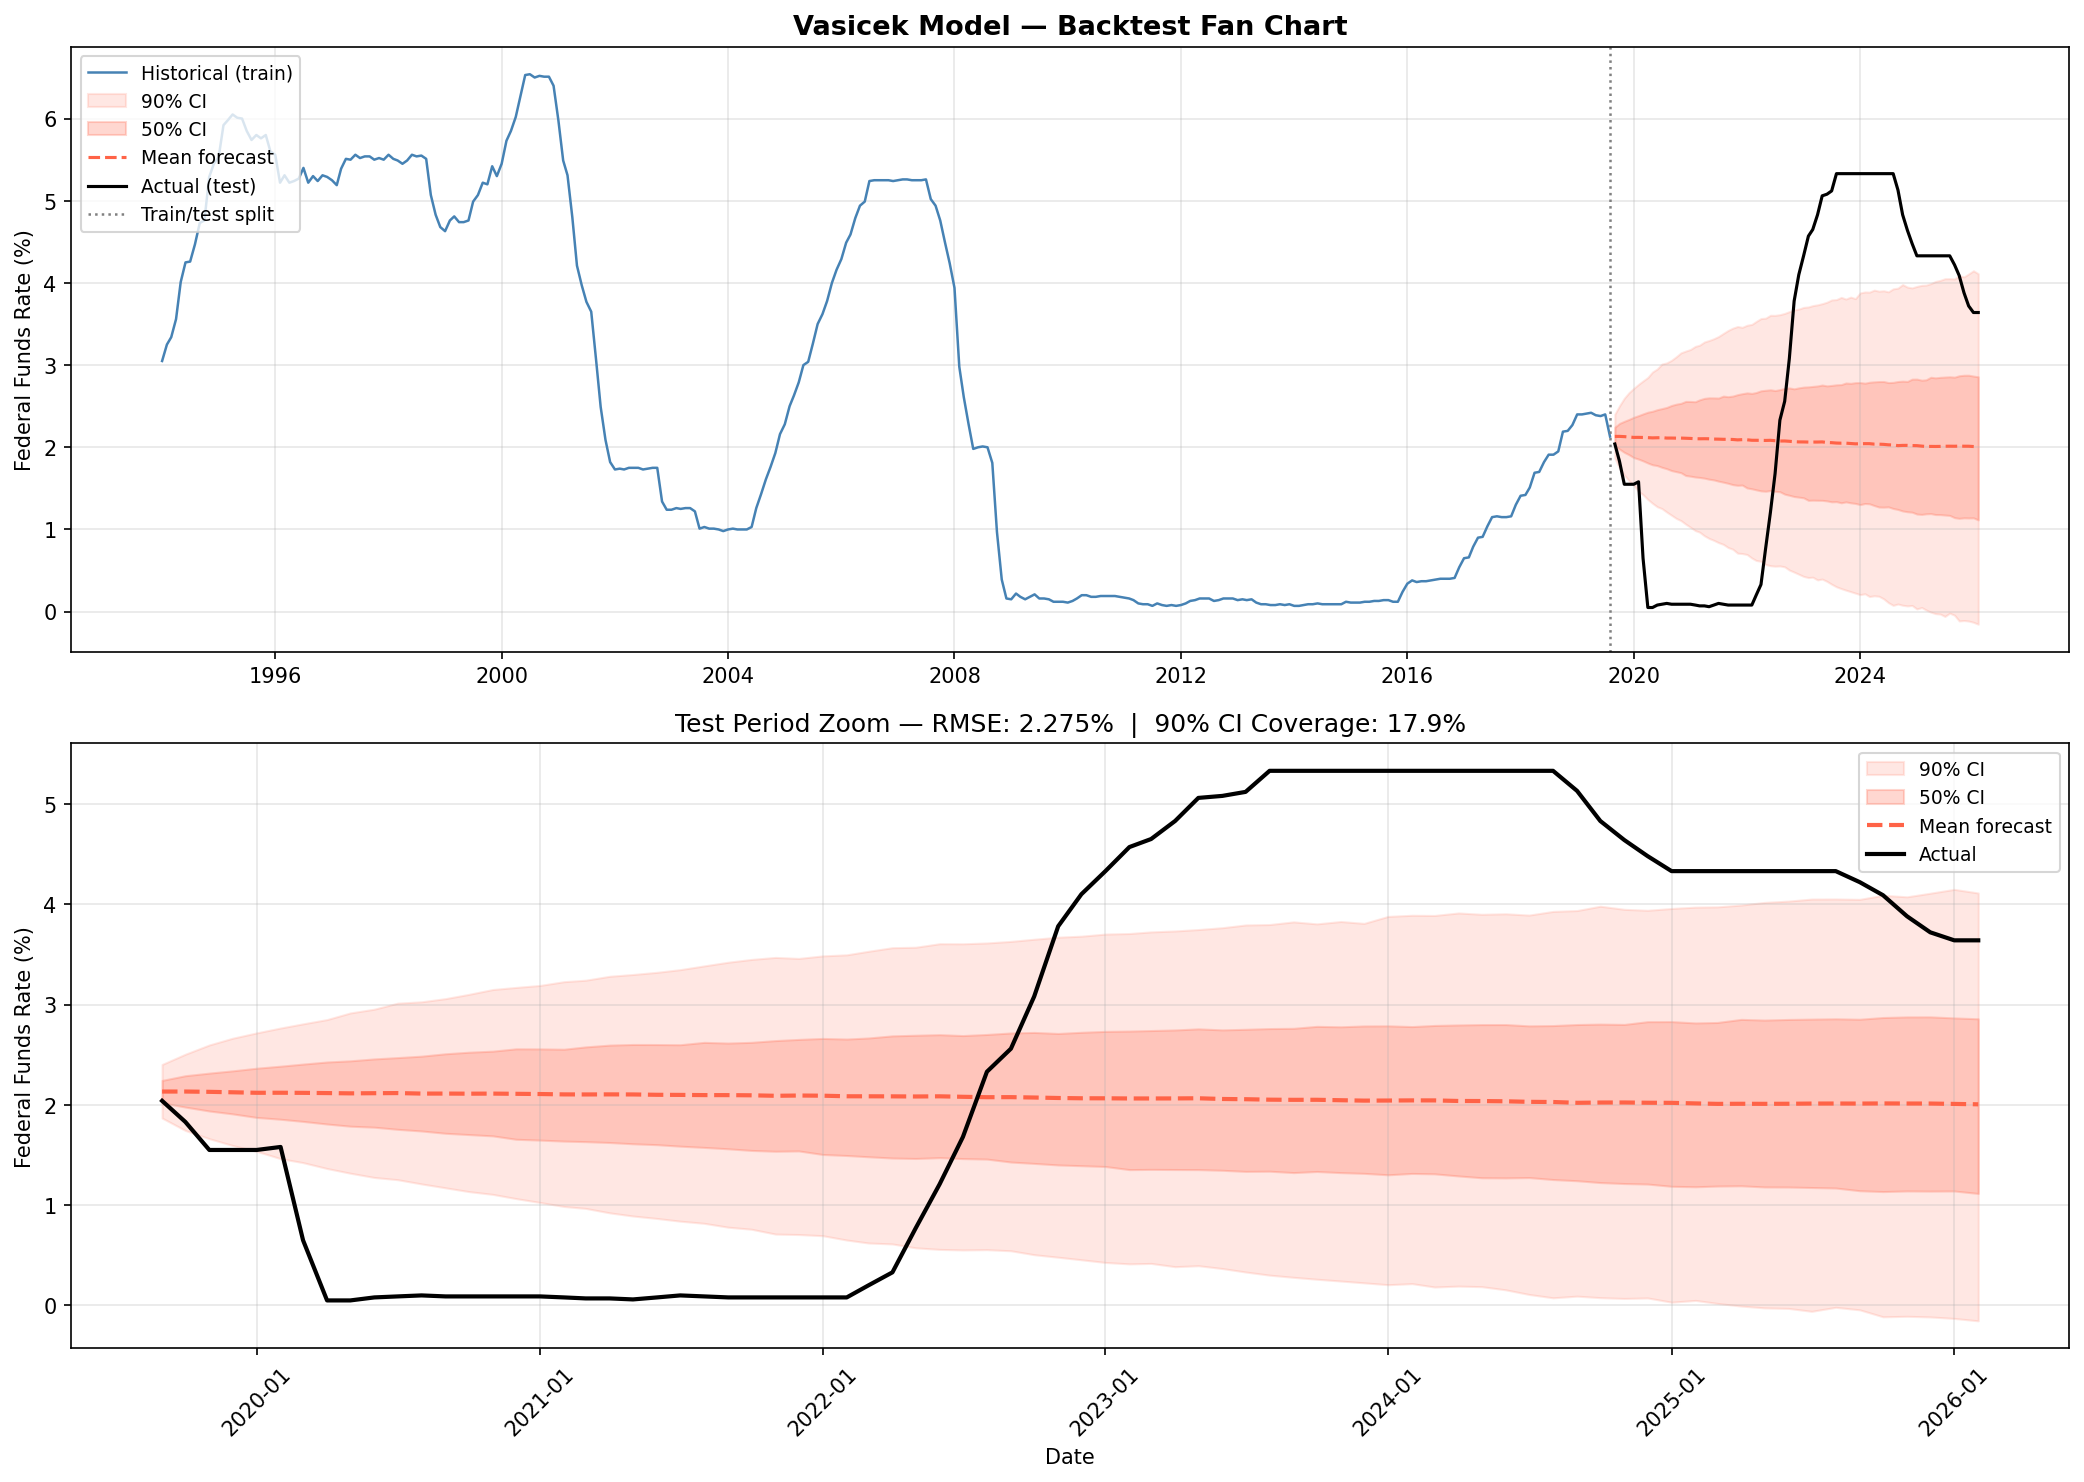
\includegraphics[width=0.95\textwidth]{backtest.png}
  \caption{Real data --- Backtest fan chart. Top panel: full history
    (1994--2026) with the forecast fan overlaid from the train/test split.
    Bottom panel: test period zoom (Sep 2019 -- Feb 2026). The actual rate
    (black) exits the confidence bands as COVID and the 2022 hike cycle unfold.
    RMSE $= 2.27\%$, coverage $= 17.9\%$.}
\end{figure}

% ══════════════════════════════════════════════════════════════════════════════
\section{Discussion and Limitations}
% ══════════════════════════════════════════════════════════════════════════════

\subsection{Why is the Vasicek Model Still Used?}

Despite its known limitations, the Vasicek model remains widely used because:

\begin{itemize}
  \item \textbf{Analytical tractability:} bond prices and option prices have
        closed-form solutions.
  \item \textbf{Interpretable parameters:} $\kappa$, $\theta$, $\sigma$ have
        clear economic meaning.
  \item \textbf{Foundation for extensions:} CIR, Hull-White, and multi-factor
        models all extend the Vasicek framework.
\end{itemize}

In practice, the Vasicek model is used for \textbf{scenario analysis} and
\textbf{relative value} rather than point forecasting. A practitioner would
ask: ``given our calibrated uncertainty bands, what is the worst-case rate
scenario at the 95th percentile?''

\subsection{Summary of Results}

\begin{center}
\begin{tabular}{@{}L{3.8cm}C{2.8cm}C{3cm}C{1.8cm}L{3cm}@{}}
  \toprule
  \textbf{Experiment} & \textbf{Oracle Coverage} & \textbf{Backtest Coverage} & \textbf{RMSE} & \textbf{Conclusion} \\
  \midrule
  Synthetic data        & 90.6\% & 59.5\% & 3.30\% & Code correct; gap = kappa bias \\
  Real data (1994--2026) & ---   & 17.9\% & 2.27\% & Regime shift + kappa bias \\
  \bottomrule
\end{tabular}
\end{center}

\subsection{Recommendations for Improvement}

\begin{center}
\begin{tabular}{@{}L{3.5cm}L{10cm}@{}}
  \toprule
  \textbf{Issue} & \textbf{Recommendation} \\
  \midrule
  Kappa bias
    & Use a shorter, more recent training window (e.g., 2015--2019) to reduce
      bias from stale regime data. \\[4pt]
  Narrow bands
    & Apply bias correction to $\hat{\kappa}$ (e.g., Phillips-Yu jackknife). \\[4pt]
  Regime shifts
    & Use a regime-switching Vasicek model with separate
      $(\kappa, \theta, \sigma)$ per regime. \\[4pt]
  Single factor
    & Extend to a two-factor model (e.g., Hull-White two-factor) to capture
      short and long rate dynamics independently. \\[4pt]
  Negative rates
    & Replace with the Cox-Ingersoll-Ross (CIR) model:
      $dr = \kappa(\theta - r)\,dt + \sigma\sqrt{r}\,dW$ --- cannot go
      negative. \\
  \bottomrule
\end{tabular}
\end{center}

% ══════════════════════════════════════════════════════════════════════════════
\section{References}
% ══════════════════════════════════════════════════════════════════════════════

\begin{enumerate}
  \item Vasicek, O. (1977). An equilibrium characterization of the term
        structure. \textit{Journal of Financial Economics}, 5(2), 177--188.

  \item Cox, J.~C., Ingersoll, J.~E., \& Ross, S.~A. (1985). A theory of the
        term structure of interest rates. \textit{Econometrica}, 53(2), 385--408.

  \item Hull, J., \& White, A. (1990). Pricing interest rate derivative
        securities. \textit{Review of Financial Studies}, 3(4), 573--592.

  \item Phillips, P.~C.~B., \& Yu, J. (2009). Maximum likelihood and Gaussian
        estimation of continuous time models in finance. In T.~G. Andersen
        et al.\ (eds.), \textit{Handbook of Financial Time Series}. Springer.

  \item Federal Reserve Bank of St.\ Louis. \textit{Federal Funds Effective
        Rate [FEDFUNDS].} Retrieved from FRED:
        \url{https://fred.stlouisfed.org/series/FEDFUNDS}
\end{enumerate}

\end{document}
